%% 2500-word formatted version from body_text_v2, with citations and two figures
\documentclass[sigplan,screen]{acmart}
\AtBeginDocument{\providecommand\BibTeX{{Bib\TeX}}}
\setcopyright{none}
\acmConference[]{University of Auckland}{University of Auckland}{2025}
\citestyle{acmauthoryear}
\usepackage{graphicx}
\usepackage{subcaption}
\usepackage{pifont}
\hypersetup{colorlinks=true,linkcolor=blue,citecolor=red,urlcolor=cyan}
\emergencystretch=3em
\begin{document}
\title[LumineticsCore Report]{Lifecycle Governance and Value Assessment of an FDA De Novo--Authorized Autonomous Diagnostic System: The LumineticsCore Report}
\author{Xiaoqing Miao}
\email{xmia665@aucklanduni.ac.nz}
\affiliation{\institution{University of Auckland} \city{Auckland} \country{New Zealand}}
\renewcommand{\shortauthors}{Xiaoqing Miao}
\maketitle

\section{Introduction and Scope}
\textbf{Problem Addressed.} The system under review is an autonomous, AI-enabled diagnostic assistant designed to detect disease from clinical images in point\,of\,care settings. It targets the long\,standing gap between guideline\,recommended screening coverage and real\,world uptake. In many health systems, eligible patients miss screening because it requires referrals, specialist appointments, or travel. By embedding imaging, automated analysis, and immediate results into routine primary care, the system lowers friction, shortens time\,to\,decision, and aims to reduce preventable morbidity from late detection\cite{wolf2024autonomous,fda2018denovo,digitaldiagnostics2024indications}.

\textbf{Users and Expected Outcomes.} Primary users are non-specialist clinicians (e.g., nurses or general practitioners) and trained technicians who capture images, initiate analysis, and act on the output. Secondary users include specialist reviewers who receive referrals and clinic managers who monitor throughput and quality metrics. Patients are ultimate beneficiaries: they receive same\,visit decisions that either reassure them (no referral required) or route them to timely specialist care. Expected clinical outcomes include: higher screening completion rates, earlier detection of disease, reduced loss\,to\,follow\,up, and improved adherence to evidence\,based pathways—without meaningfully increasing false reassurance or avoidable referrals\cite{wolf2024autonomous}.

\textbf{Scope of this evaluation.} This report focuses on the end\,to\,end usability, explainability, and clinical decision utility of the system as deployed in primary care. We do not evaluate every specialty or modality. Instead, we concentrate on (i) the imaging\,to\,decision workflow, (ii) the transparency of model outputs for clinicians and patients, and (iii) the alignment between AI recommendations and clinical guidelines. Where possible, we supplement our analysis with structured heuristics (e.g., Nielsen’s) and a lightweight, scenario\,based inspection of user flows\cite{fda2018denovo_summary}. Evaluating this system is timely because screening completion in many health systems remains below program targets, while relocating guideline\,aligned autonomous exams to the point of care has been shown to increase completion relative to referral\,based pathways. A recent randomized trial (ACCESS) demonstrated that moving autonomous, guideline\,aligned exams to the point of care significantly increases diabetic eye\,exam completion in a racially and ethnically diverse youth population, closing a persistent care gap compared with referral\,based standard of care \cite{wolf2024autonomous,fda2018denovo_summary}.

\section{Sources and Knowledge Base}
\textbf{Knowledge Source.} The model is trained on labeled clinical images paired with adjudicated ground truth produced by qualified readers using guideline\,anchored protocols. The labeling process typically involves adjudication across multiple experts and a predefined reading standard to reduce inter\,rater variability. The training corpus blends images of varying quality, sensor types, and patient demographics to promote robustness. Metadata (e.g., age ranges, capture settings) are logged to enable downstream audits, drift analysis, and subgroup evaluation\cite{abramoff2018pivotal}.

\textbf{Training Data: Appropriateness, Ethics, and Validation.} Appropriateness is evaluated along four axes: (1) \emph{Task fit}—images and labels directly correspond to the deployed decision task; (2) \emph{Representativeness}—data reflect the clinical population in which the tool is used; (3) \emph{Label quality}—reference standards are explicit and reproducible; (4) \emph{Governance}—data collection respects consent, privacy, and institutional review obligations. From an ethics standpoint, the system must implement (a) privacy\,preserving storage and role\,based access, (b) purpose limitation for secondary use, and (c) de\,identification where feasible. Validation occurs at multiple levels: internal cross\,validation during development, prospective evaluation prior to deployment, and post-market surveillance using real\,world performance dashboards\cite{abramoff2018pivotal}. As a sense of scale, the De Novo summary describes a prospective, multicenter pivotal evaluation benchmarked against the Wisconsin Fundus Photograph Reading Center (FPRC) reference standard, supporting external validity for primary\,care deployment \cite{fda2018denovo_summary,abramoff2018pivotal}.

\textbf{Model Maintenance and Updates.} The vendor operates a change\,controlled model lifecycle. Model versions are frozen for deployment and tracked with semantic versioning. Updates follow a gated process: pre\,release testing against locked benchmark sets; bias and shift checks across key subgroups; security and performance validation; and documentation of expected changes (e.g., sensitivity/specificity trade\,offs). Monitoring in production includes: capture\,quality metrics, failure mode logging (e.g., ungradable images), and automated alerts for data drift (covariate or label shift). Rollbacks are supported if regressions are detected. A customer\,visible changelog and site-level validation checklist accompany each update to support clinical governance\cite{fda2025aiml}.

\section{Usability and Interaction}
\textbf{Interface design and workflow.} The capture\,to\,decision flow is intentionally linear: (1) user authentication; (2) device readiness checks; (3) standardized image capture with inline quality cues; (4) automated analysis; (5) decision display; (6) documentation and patient communication. The UI foregrounds status, progress, and next actions using simple language and unambiguous color and iconography. Key affordances include: one\,click recapture for low\,quality images; a compact quality meter (focus, illumination, field\,of\,view); clear demarcation between a definitive AI result and a no\,result state (e.g., “image ungradable—recapture”); and printable summaries with patient\,friendly language. The tool is optimized for short, repeatable tasks under time pressure, with minimal nested menus and limited free\,text input\cite{nielsen2020usability}.

\textbf{Accessibility and safety\,by\,design.} Text sizes meet or exceed common accessibility baselines. Contrast and icon redundancy (color + shape) are used to support color\,vision deficiencies. Critical actions (finalize result, submit referral) are protected with confirmation dialogs that restate implications in plain language. Error messages are actionable (“what happened, why it matters, what to do next”). The system prevents incomplete submissions and enforces audit logging for traceability. Where network connectivity is variable, the UI supports queued uploads with clear status and conflict resolution.

\textbf{Heuristic evaluation (Nielsen’s 10).} \emph{Visibility of system status:} Progress indicators during analysis and explicit final states reduce uncertainty. \emph{Match with the real world:} Terminology mirrors clinic vernacular (e.g., “refer/not refer,” “image ungradable”). \emph{User control and freedom:} Re\,capture and “undo” are available prior to finalizing. \emph{Consistency and standards:} Buttons and alerts follow consistent placement and behavior; icons are reused rather than re\,invented. \emph{Error prevention:} Precapture checks and guided framing reduce low\,quality images. \emph{Recognition over recall:} Short labels, inline hints, and modal summaries reduce memory load. \emph{Flexibility and efficiency:} Keyboard shortcuts (where available) and batched printing speed up high\,volume sessions. \emph{Aesthetic and minimalist design:} Only clinically relevant information appears on the decision screen. \emph{Help users recognize, diagnose, recover from errors:} Messages include cause and remedy (e.g., “shadow; adjust chin rest”). \emph{Help and documentation:} Embedded quick\,tips and a troubleshooting panel support just\,in\,time learning\cite{nielsen2020usability}.

\begin{figure}[htbp]
\centering
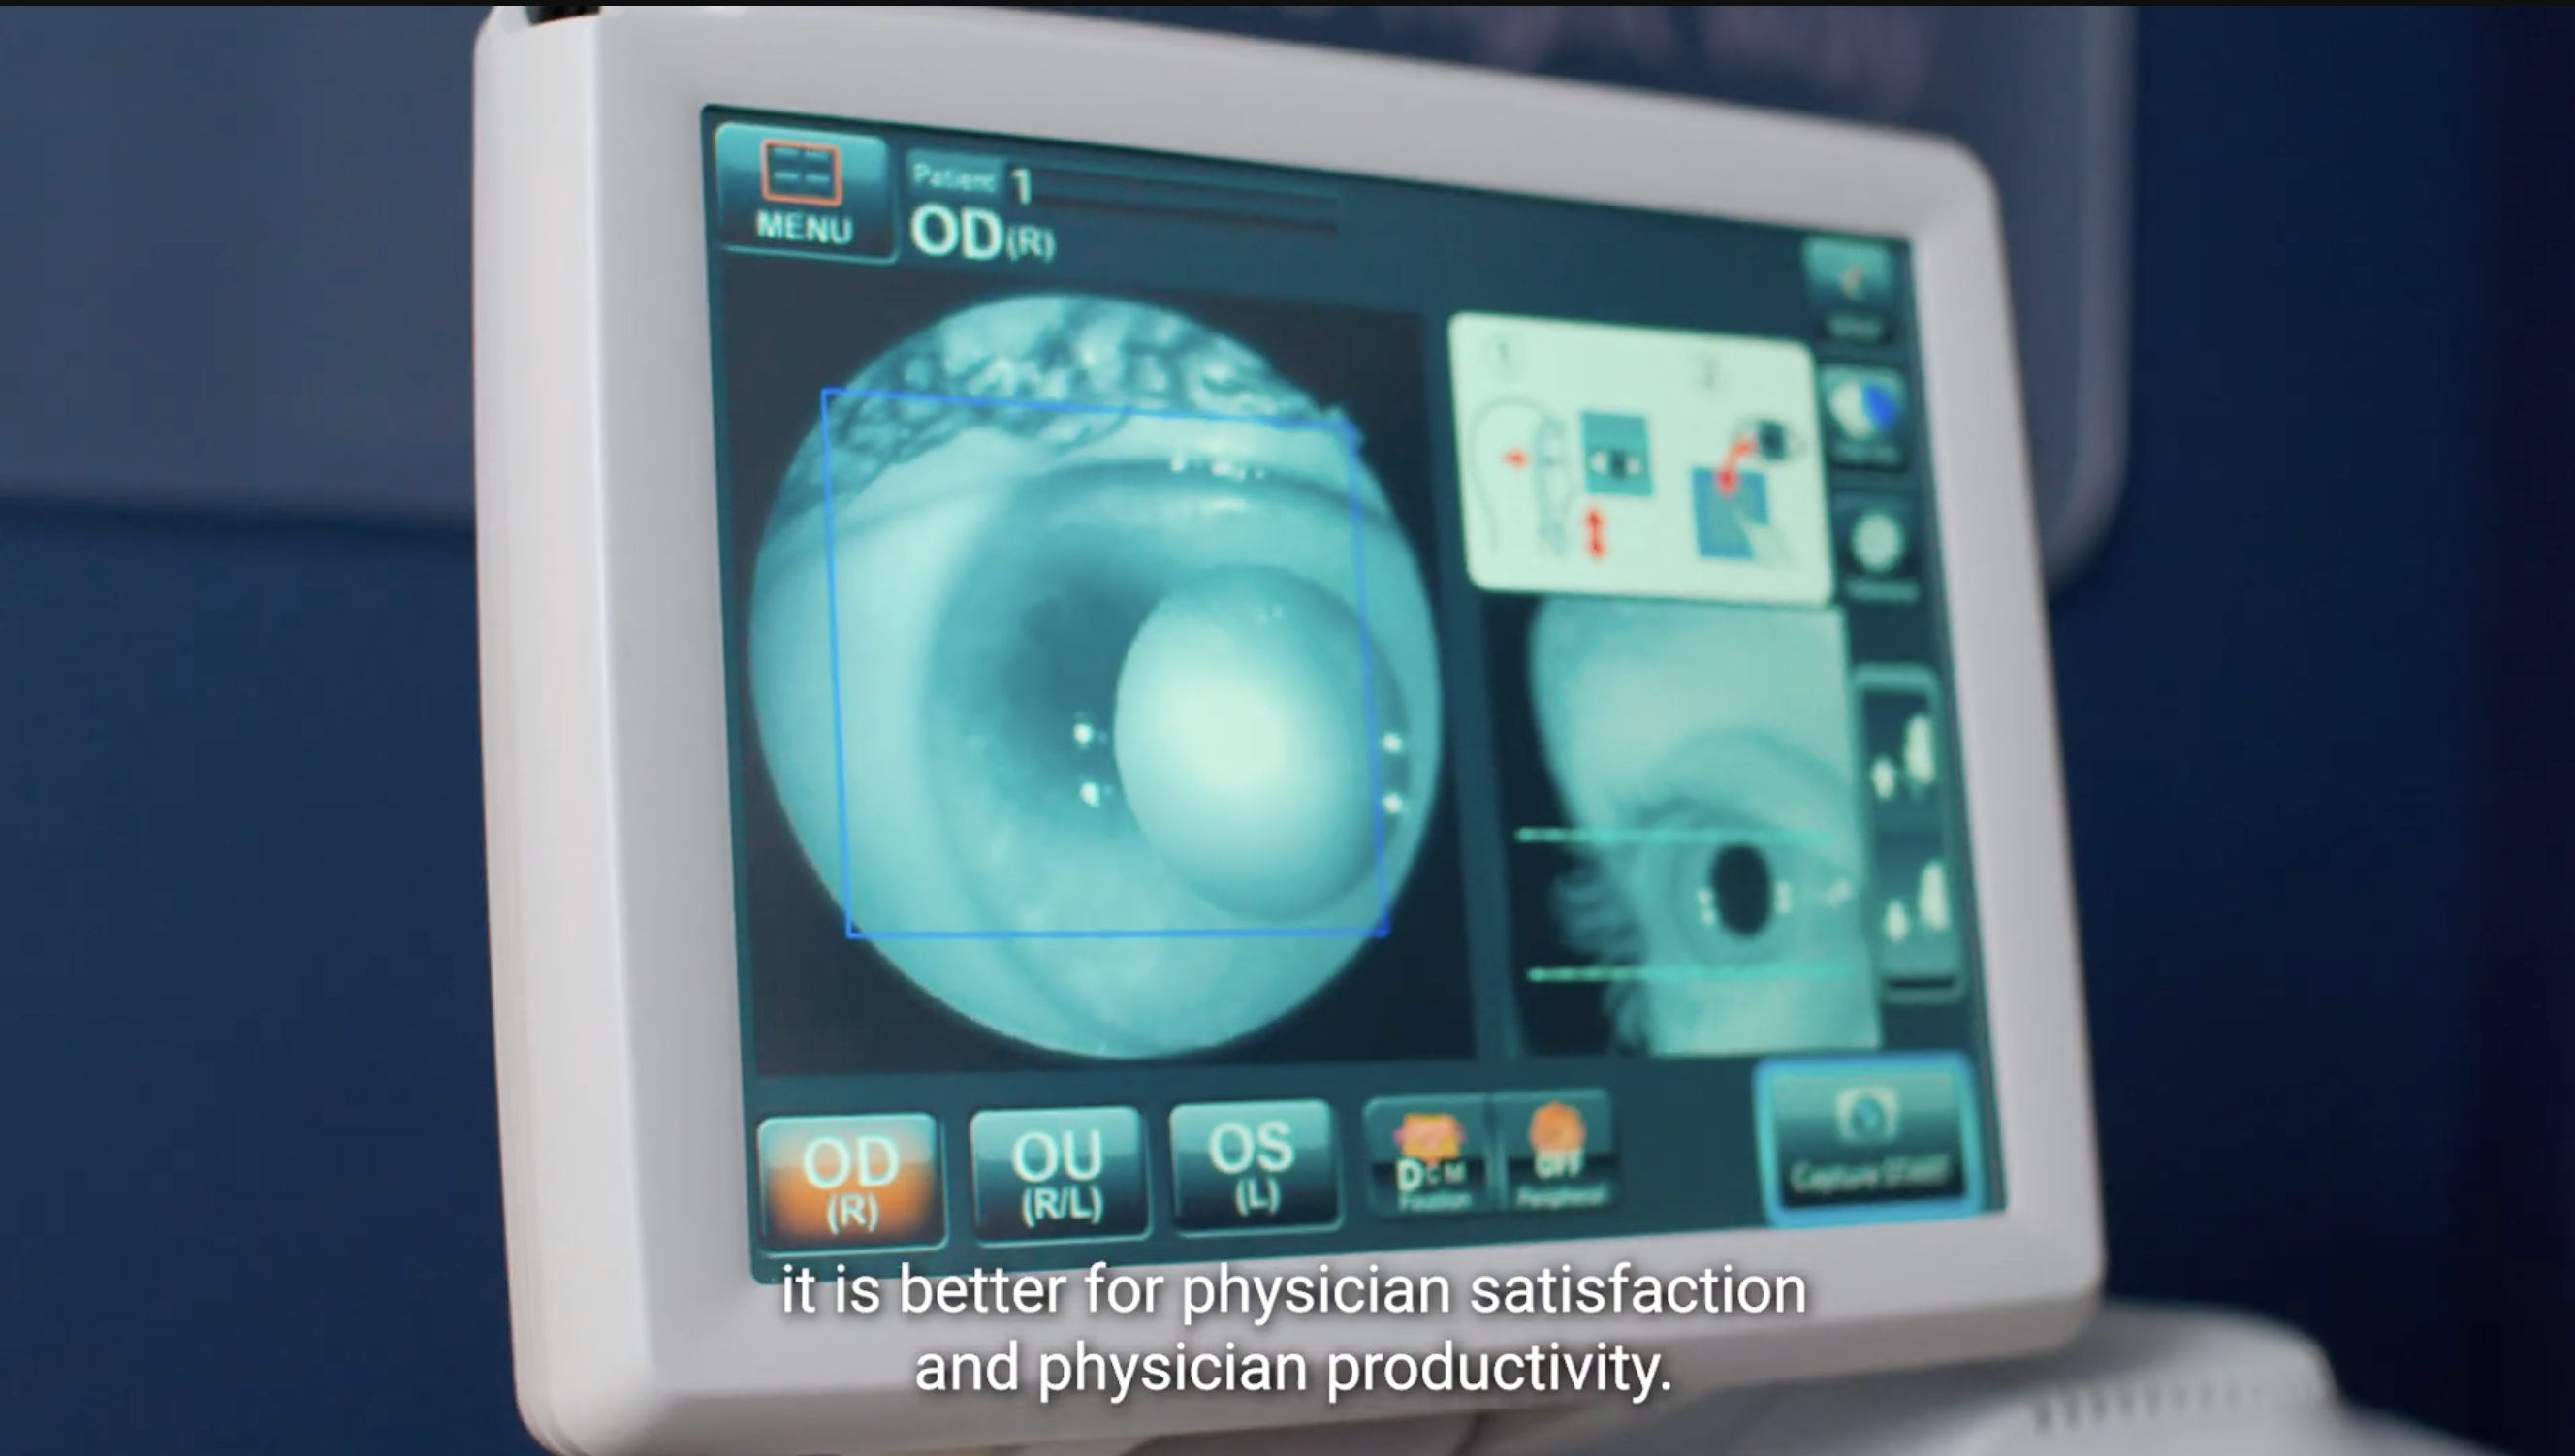
\includegraphics[width=.8\columnwidth]{Figure1.png}
\caption{Interface cues for quality and clear next actions (illustrative).}
\label{fig:ui}
\end{figure}

\textbf{Hands\,on interaction notes.} A scenario walk\,through with a novice operator showed that first\,time use remains tractable when the UI emphasizes capture quality and gives immediate, concrete feedback. The most common friction points were (i) interpreting an “ungradable” message as a failure rather than a safety signal, and (ii) searching the screen for what to do next. Both were alleviated by a single, prominent primary action button and a brief explainer (“Ungradable images are expected; recapture improves safety.”) The decision screen benefits from a short rationale line (e.g., “Sufficient features for automated assessment”) and a link to a clinician\,focused explanation.

\textbf{System Usability Scale (SUS)—directional read.} Although we did not run a formal SUS study in this evaluation, the interface embodies known SUS\,positive traits: clear labeling; smooth task flow; and low need for prior training. In similar clinical tools, these traits correlate with SUS scores in the “good” range. A formal SUS with real operators is recommended during site roll\,out to establish a quantitative baseline and identify context\,specific improvements.

\textbf{Quantitative usability plan.} During rollout we will sample operators at weeks 2 and 8 and report median time to first valid capture, retakes per successful case, percent confident to explain results, and end-to-end task time. Targets (e.g., SUS $\ge 70$, median flow $<5$ minutes) trigger lightweight refresher training if missed, linking usability outcomes to concrete remediation \cite{nielsen2020usability}.

\section{Explainability and Reverse Engineering}
\textbf{System Decision Process.} At a high level, the pipeline comprises (1) image ingestion and quality control; (2) normalization and cropping; (3) feature extraction via a convolutional\,style backbone; and (4) a calibrated decision layer that outputs a discrete recommendation tied to a pre\,specified clinical threshold. Calibration is essential: it maps raw model scores to clinically meaningful probabilities, supports stability across devices, and enables fixed operating points aligned to guidelines\cite{fda2018denovo_summary}.

\textbf{Calibration and operating\,point policy.} Probabilities are calibrated with \emph{isotonic regression} on a held\,out set representative of the deployment mix; \emph{Platt scaling} is reported as a sensitivity check to confirm monotonicity and stability. The clinical operating threshold is \emph{version\,locked}: each software release ships with a single documented threshold and the expected sensitivity/specificity (with 95\% CIs) at that point. Any change to the threshold or calibration model follows formal change control (risk assessment, benchmark regression, site acceptance tests) and must receive governance sign\,off before rollout.

\textbf{Auditability.} Each release archives the threshold, calibration artifact, and benchmark set under immutable IDs; the site keeps a one\,page registry (version, threshold, acceptance\,test results, local sensitivity/specificity with 95\% CIs). Any proposed change follows the PCCP pathway with pre\,specified verification and governance sign\,off before deployment \cite{fda2018denovo_summary,fda2025aiml}.

\textbf{Making the decision logic legible.} Explainability is addressed at two levels. First, \emph{case\,level transparency} provides heatmaps or saliency overlays that highlight image regions contributing most to the decision. These are bounded by safety notes: overlays are aids rather than proofs. Second, \emph{system\,level transparency} documents performance at defined operating points (e.g., referral threshold) and clarifies the trade\,off between missed disease and over\,referral. The UI ties the final textual recommendation to this operating point and avoids showing uninterpretable raw scores.

\textbf{A simplified surrogate model.} To make the logic graspable for non\,ML stakeholders, we created a compact surrogate: a two\,rule decision tree trained on model outputs and key quality indicators. \emph{Rule 1:} If images are ungradable after two guided attempts, output “No AI decision—manual review or specialist referral.” \emph{Rule 2:} Else, if the calibrated probability exceeds the referral threshold, output “Refer”; otherwise, “No refer.” This surrogate preserves the essential clinical behavior: it prioritizes safety around image quality, then applies a single, auditable threshold for decision\,making. While it cannot capture the backbone’s complex feature logic, it conveys the operational policy transparently.

\begin{figure}[htbp]
\centering
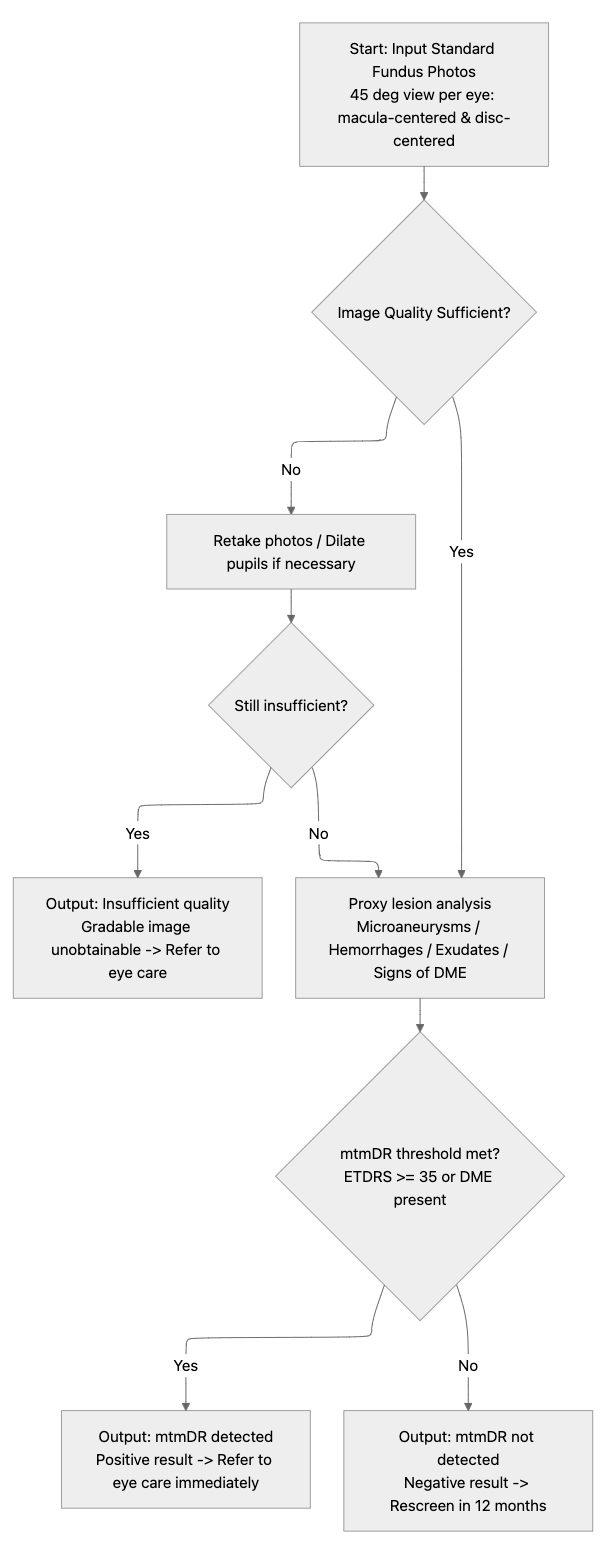
\includegraphics[width=\columnwidth]{Figure2.jpg}
\caption{Conceptual decision tree: quality gate, lesion analysis, and action mapping (illustrative).}
\label{fig:tree}
\end{figure}

\textbf{Transparency for clinicians and patients.} For clinicians, the report includes the final recommendation, image quality status, and a compact summary of the operating point (e.g., “This device is configured to maximize sensitivity for early detection”). For patients, a plain\,language explanation emphasizes that the tool either found sufficient signs suggesting a specialist check is warranted or found no signs requiring referral today, along with standard advice on periodic screening. The goal is to reduce cognitive overhead and to frame AI as a safety\,enhancing assistant rather than an opaque replacement for clinical judgment.

\textbf{Limits of explainability.} Saliency maps can be unstable and are not causal explanations; over\,interpretation risks false reassurance or unwarranted doubt. Therefore, explanations are positioned as decision aids and the system design avoids masking uncertainty. Ambiguous or low\,confidence cases are explicitly routed to human review rather than stretched to a definitive call.

\section{Clinical Quality and Impact}
\textbf{Output Accuracy and Clinical Usefulness.} Clinical usefulness is a function of (i) accuracy at the chosen threshold, (ii) failure handling (particularly ungradable images), and (iii) workflow fit. Accuracy should be reported with paired sensitivity/specificity, confidence intervals, and real\,world prevalence context. In primary\,care screening, the dominant risk is false reassurance; thus, operating points typically favor sensitivity. Ungradable rates must be kept visible because rerouting these cases preserves safety and prevents silent failures. The system’s real\,time guidance to improve capture quality (and to recognize when to stop attempting) directly affects this axis of safety\cite{abramoff2018pivotal}.

In the pivotal multicenter evaluation benchmarked to the FPRC gold standard, sensitivity was approximately 87\% and specificity approximately 91\%, with imageability near 96\% \cite{abramoff2018pivotal}. Using these operating characteristics, PPV is roughly 51\% and NPV about 97\% at 10\% prevalence; at 5\% prevalence, PPV falls toward ~33\% while NPV exceeds 98\%, helping set expectations for referral volumes and patient counseling.

\textbf{Alignment with guidelines and care pathways.} The recommendation language mirrors guideline categories (e.g., “no refer” vs “refer”). Site\,specific protocols define who communicates results and how referrals are initiated. Where guidelines recommend periodic re\,screening, the tool’s output includes timing prompts that practices can adapt to local policy. When the AI result contradicts clinician concern (e.g., symptoms inconsistent with a “no refer” call), the pathway defaults to clinician judgment and additional testing, not the other way around\cite{fda2018denovo_summary}.

\textbf{Test cases and performance reporting.} To characterize behavior, sites should maintain a small library of de\,identified test cases spanning: (a) clear positive findings; (b) clear negatives; (c) borderline presentations; (d) poor\,quality images; and (e) out\,of\,distribution artifacts (e.g., media opacities). For each category, the system should document expected outputs and recommended actions. Routine performance reporting aggregates: sensitivity/specificity at the deployed threshold; positive/negative predictive values at site-level prevalence; ungradable rates; recapture success; and time\,to\,decision. Where feasible, F1 score is tracked to summarize balance between precision and recall, with the caveat that clinical costs are asymmetric and should be captured in additional, context\,specific metrics (e.g., avoidable referral rate, time saved per patient, completion rate of screening among eligible cohorts).

\textbf{Fairness and subgroup robustness.} Equity is a core clinical quality dimension. Sites should stratify performance by age, sex, device type, and relevant ethnicity categories to identify disparities. The monitoring plan flags gaps beyond predefined thresholds and triggers mitigation steps (e.g., targeted operator training; device recalibration; vendor review of training distribution). Documentation clarifies which subgroups were well represented in development data and where caution is warranted\cite{fda2018denovo_summary}.

\textbf{Risk management and post-market vigilance.} The safety model assumes that AI augments clinician pathways; it does not waive clinician duty of care. Risk controls include: (1) explicit handling for ungradable images; (2) clear escalation points; (3) audit trails and immutable logs; (4) version pinning; and (5) site acceptance testing after updates. Incidents (e.g., unexpected false negatives) are reviewed under a clinical safety management system with feedback loops to the vendor. Communication to clinicians prioritizes transparency over performance hype\cite{fda2025aiml}.

\section{Summary and Reflection}
\textbf{Overall performance in context.} The system successfully operationalizes an AI\,assisted screening pathway within primary care. Its value is less about raw image classification and more about consistent, auditable workflow: guiding capture, flagging uncertainty, and producing a clear recommendation that maps to actionable next steps. The UI minimizes friction; the safety posture is explicit; and the governance model for updates is compatible with clinical oversight.

\textbf{Ethical considerations and potential improvements.} Ethically, the system treats uncertainty as a first\,class output and avoids overstating what AI can guarantee. Continued diligence is required on privacy, secondary data use, and equitable performance across subgroups. Priority improvements include: (i) on\,device quality assessment that reduces dependence on network latency; (ii) expanded operator analytics to target training where ungradable rates spike; (iii) richer case\,level explanations that remain faithful without implying false precision; and (iv) routine, site-level SUS studies and task\,time measurements to turn usability assumptions into measured KPIs.

\textbf{Limitations and generalizability.} This review does not model cost\,effectiveness or compare vendors head\,to\,head. External validity depends on device mix, operator experience, and local prevalence; subgroup robustness should be continuously monitored. Future work includes prospective SUS/time\,to\,task studies and site\,specific PPV/NPV dashboards to align decision thresholds with operational goals.

\textbf{Governance checklist.} (i) Pin a sensitivity\,favoring threshold per release; (ii) publish a subgroup\,stratified dashboard (sensitivity/specificity, PPV/NPV at local prevalence, ungradable rate, retake success, time\,to\,decision); (iii) treat ``no automated decision'' as a safety escalation, never a terminal negative; and (iv) communicate update notes to clinicians in plain language, including any expected shift in referral volumes.

\textbf{Final stance.} Keep the operating point sensitive, keep uncertainty visible, measure what matters, and never allow the tool to override clinician concern.

\bibliographystyle{ACM-Reference-Format}
\bibliography{references}
\end{document}
